\documentclass{article}
\usepackage{amssymb}
\usepackage{pdfpages}
\usepackage{hyperref}
\usepackage{cleveref}
\usepackage{enumitem}
% set the margin of the document
\usepackage[a4paper, total={7in, 10in}]{geometry}

\hypersetup{
	colorlinks=true,
	allcolors=blue,
}

\renewcommand{\thesubsection}{\thesection.\Alph{subsection}}


\begin{document}
\begin{titlepage}
   \vspace*{270px}
  \begin{center}

    \Large\textbf{CS446 Deliverable 1 - Project Proposal}

   \vspace{50px}

    \Large{Project Title: Pitch-Perfectly-Accurately Practice}

   \vspace{50px}

    \large{Irvine Yao (b6yao)\\Jialin Shan (j6shan)\\Alex Lai \ (x7lai)\\Johnny Gao (z53gao)}

  \end{center}
\end{titlepage}
  
% set global enumerate line space
\setlist[enumerate]{topsep=0pt,itemsep=-1ex,partopsep=1ex,parsep=1ex}.
% set global itemize line space
\setitemize{noitemsep,topsep=0pt,parsep=0pt,partopsep=0pt}


\section{Introduction}
\label{sec:introduction}
\qquad
		With the growing popularity of music related platforms such as TikTok and singing live streams, more and more people are interested in singing and want to learn it.
		Many of them realize that in order to sing beautifully on the right keys and notes, they need to train their listening and singing skills in order to have perfect pitch. 
		Perfect pitch is a skill that let people recognize the pitch of any sound, a skill that every musician dreams to have. 
		Possessing perfect pitch not only can help you to develop the ability and confidence to sing on pitch, but is also a key factor for a good musician. 
		In order to have this skill, musicians usually have to practice for many years. 
		One way is to sing a note and then adjust their singing based on how that note should sound on a tuned instrument. 
		So for the longest time, people need to have access to a tuned instrument in order to practice, as well as hiring a singing coach to help you practice and give you feedback, which can be very inconvenient and expensive. 
		With the advancement of the technology, computational device is getting incredibly cheap and portable. 
		Nearly everyone today has a smartphone, so we are planning to assist people who want to practice perfect pitch whenever and wherever they want by developing a mobile application called Pitch-Perfectly Accurately Practice (PPAP). 

\qquad

		PPAP is an Android application that help you to practice perfect pitch skill by singing to your phone.
		After you download PPAP, you can start to practice right away. 
		The app takes advantage of smartphones’ multi-touch screen and advanced display technology. 
		We plan to give our app simplistic and intuitive UI that give you real-time feedback for your singing, so you can adjust your singing accurately. 
		While singing to your phone, PPAP will detect the current sound frequency of your voice to give you a precise feedback on how low or high you are compare to the correct notes. 
		It’s like having a singing coach with you all the time without costing you a single dime. 
		Outside of note practicing, PPAP can also helps you to recognize and reproduce intervals and chords, both of which are essential for musicians. 
		For singers trying to practice songs, PPAP has song practice mode with suitable metronome and real-time sounds detection that helps you to practice your favourite songs from our songs library.

\qquad

		With real-time sound frequency detection, real-time feedbacks on a intuitive UI, made possible by the microphones, speakers and multi-touch screen that every smartphones has. We believe PPAP is the easiest way for people to practice perfect pitch.

\section{Functional Properties}
\label{sec:function_properties}
\subsection{Overview}
\label{subsec:overview}
\begin{enumerate}
  \item \label{itm:tutorial} A walk-through tutorial at first launch about features in the app
  \item \label{itm:left_menu} \textbf{Left Menu} button on the top-left corner brings out \textbf{Left Menu} to select practice mode (can also be triggered by swiping from left)
  \item \label{itm:help} \textbf{Help}(?) button on the bottom-left corner to spawn a help page for each practice mode
  \item \label{itm:play_sound_general} \textbf{Play Sound} button on the top-right corner to play the \textit{answer} note
  \item \label{itm:filter_general} \textbf{Filter}(F) button on the bottom-left corner to spawn a \textbf{Filter Menu} where questions are generated from the set of notes $S$ that the user selects. It contains \textit{filter}s: \textit{From and To}, \textit{Key Signature and Scale}, using those \textit{filters} a set of notes $S$ will be listed below. The user can slide down to (un)select or (un)select all or select complement.
  \item \label{itm:setting_menu} \textbf{Setting Menu} can be accessed from "Left Menu", it contains toggle for \textit{metronome}, slider for \textit{error allowance} level, slider for \textit{in-app volume}, option for \textit{theme}.
  \item \label{itm:more_menu} \textbf{More Menu} can be accessed from \textbf{Left Menu}, it contains \textit{Summary}, \textit{Music Theory}, \textit{FAQ}, \textit{About us}, \textit{Donate}, \textit{Contact us} sections.
  \item \label{itm:summary} \textit{Summary} section in \textbf{More Menu} contains a graph summary of the accuracy of the notes you practiced, top ten notes you mastered and notes on notes you need to work on. 
  \item \label{itm:double_tap_next_question} Double tap on screen to skip to next question (again generated by the set of notes $S$ user can select).
\end{enumerate}

\subsection{Note Practice Mode}
\label{subsec:note_practice_mode}
\begin{enumerate}
  \item\label{itm:question_note} Generate a \textit{question} ``$X$'' on screen, where $X$ is a note, the user is supposed to sing that note. 
  \item\label{itm:detection_note} If the user produces no sound for a certain time, the text box will show "Please sing..." or "...". If the user sings too low, $\uparrow\uparrow$ will bounce rapidly displayed above the note. If the user sings almost but still low, $\uparrow$ will bounce slowly. $\downarrow\downarrow$ and $\downarrow$ will be shown below the note in the opposite cases. If the user sings the correct note within \textit{error allowance range}, $\checkmark$ shows above the note.

\end{enumerate}

\subsection{Interval Practice Mode}
\label{subsec:interval_practice_mode}
\begin{enumerate}
  \item \label{itm:question_interval} Generate a \textit{question} ``$X + K$'' on screen, where $X$ is the key signature, $K$ is a interval (e.g. M5, can be negative). The user is supposed to sing the note that $K$ above/below $X$.
  \item \label{itm:detection_interval} Same as \ref{subsec:note_practice_mode}.\ref{itm:detection_note}
  \item \label{itm:play_sound_interval} \textbf{Play sound} button behaves differently, where long press plays correct \textit{answer} $X+K$ and short release to play $X$.

\end{enumerate}

\subsection{Chord Practice Mode}
\label{subsec:chord_practice_mode}
\begin{enumerate}
  \item \label{itm:question_chord} Generate a set of notes $Z$ on screen, where $Z$ contains notes from a chord $H$ generated by $S$ from \textbf{Filter Menu}. 
  \item \label{itm:detection_chord} Individual notes in $Z$ are evaluated individually in any order, up/down arrows or $\ldots$ or $\checkmark$ will be shown same as in \textsuperscript{\ref{subsec:note_practice_mode}.\ref{itm:detection_note}}
  \item \label{itm:filter_chord} \textbf{Filter Menu} is different than above. It contains a slider for \textit{key signature}, and checkboxs for \textit{include major, include minor, include inversion, include diminished, include maj7, include 7, include sus4, etc.}. (or something else that does the same logic)
  \item \label{itm:playsound_chord} \textbf{Play sound} button behaves differently, where short release plays chord $CEG$ and long press to play $C, E, G$ sequentially.

\end{enumerate}

\subsection{Song Practice Mode}
\label{subsec:song_practice_mode}
\begin{enumerate}
  \item\label{itm:library} \textbf{Library} button on the left pops a list of songs. (each song will be just a melody less than 30 secs)
  \item\label{itm:submodes} \textbf{Play/Practice} button on the right switches between submodes \textbf{Playing mode} and \textbf{Practicing mode}. 
    \begin{enumerate}
      \item\label{itm:playing_mode}\textbf{Playing mode}: Notes from the song will be played by grand piano. 
						\textbf{Play/Pause} button in the middle play/pause the song.
						A slider under the note can adjust the progress of the song.
						Tap \textbf{Play Sound} button to play the correct note. A metronome can be toggled in \textbf{Setting Menu}. (Toggling the metronome might reset the progress of the current playing song)
          \item\label{itm:practice_mode}\textbf{Practicing mode}: The user try to produce the note of current note, (see last page). It will proceed to next note if the user sings correctly within \textit{error allowance} range, or double tap on screen. When the user long presses on the note box, a slider will be shown under the note box (hide the text), so that the user can swipe to select, and tap elsewhere to exit this mode. A metronome can be toggled at anytime. (won't reset the progress)
    \end{enumerate}

\end{enumerate}

\section{Non Functional Properties}
\begin{enumerate}
  \item Maintainability
    \begin{itemize}
      \item Easy to maintain. The only maintenance would be to patch bugs and add modes when needed.
    \end{itemize}
  \item Reusability 
    \begin{itemize}
      \item Main pitch detection code and menu is reused for future modes
    \end{itemize}
  \item Complexity (Ease of use)
    \begin{itemize}
      \item Uses standard android UI; It should be intuitive for an averagely experienced use to navigate the app
      \item Operation should be easy as the user just needs to try and sing the note
      \item There is no dependence on servers since it is mainly offline (User experience not affected by updates or network delay).
    \end{itemize} 
  \item Evolvability
    \begin{itemize}
      \item Should easily add extra modes and custom features as they are separate except for the pitch recognition function
      \item Data tracking through cloud can be later added (Tracking is independently done and called in the modes when training)
    \end{itemize}
  \item Internationalization and localization
    \begin{itemize}
      \item Easy to add languages to settings; notes are internationally recognized
    \end{itemize}
  \item Performance 
    \begin{itemize}
      \item Should be relatively quick as it is only measuring frequency (Maybe average) to see if user sings on pitch
    \end{itemize}
  \item Usability
    \begin{itemize}
      \item User should be able to use it anywhere they are allowed to make loud noises
    \end{itemize}
  \item Availability
    \begin{itemize}
      \item Android App Store can download it (hopefully).
    \end{itemize}
\end{enumerate}

\section{Use Cases}
\subsection{Use Case 1 - Note Practice}
\qquad
		Say the user wants to practice random notes in $S$ and already in \textit{note practice mode} when the app launches. \textsuperscript{\ref{subsec:note_practice_mode}.\ref{itm:question_note}}
		If not in note practice mode, the user can swipe right from left of screen or click  the \textbf{Left Menu} button \textsuperscript{\ref{subsec:overview}.\ref{itm:left_menu}} to select the node practice mode from the menu.
    Then the app would select a random note in $S$ (e.g $A_4^\sharp$). Once they sing a note, the app will analyze the note and see if they are correct \textsuperscript{\ref{subsec:note_practice_mode}.\ref{itm:detection_note}}. 
    If they are not correct then give them an arrow to tell them to go higher or lower (The arrow will bounce faster as they are further to tell them to go much higher or lower). 
    If they are correct then it will notify them. 
    The user let the app play the note they are asked to sing \textsuperscript{\ref{subsec:overview}.\ref{itm:play_sound_general}}. 
    Once they are correct or choose to skip the note by double tapping \textsuperscript{\ref{subsec:overview}.\ref{itm:double_tap_next_question}}, they are given another note (B.2). 
    This repeats until the user decides that they no longer want to be in note mode, in that case they can close the app. 
    Their practice session information is saved in real time \textsuperscript{\ref{subsec:overview}.\ref{itm:summary}}. 
    They can view history in Summary Section in More Menu \textsuperscript{\ref{subsec:overview}.\ref{itm:more_menu}}.

\subsection{Use Case 2 - Interval Practice}
\qquad
    Interval Practice mode can be switched in the \textbf{Left menu} \textsuperscript{\ref{subsec:overview}.\ref{itm:left_menu}}. 
    The user interface of this mode is similar to that of note practice mode, the app will give the user a pitch name as well as a frequency interval higher or lower than it. 
    For example, $D_3 + M_5$ means the app is asking for the $M_5$(major fifth interval) above D3. \textsuperscript{\ref{subsec:interval_practice_mode}.\ref{itm:question_interval}} 
    Then user needs to sing that note. 
    System detects the frequency that user sings, and shows if the frequency they sing is higher or lower than the correct note using an arrow\textsuperscript{\ref{subsec:interval_practice_mode}.\ref{itm:detection_interval}}. 
    There are four buttons in this page, which are the same as the note practice page. 
    Among these buttons, the play button behaves slightly different than note practice, that is when the user long press it, system plays the correct note sound; or single pressing let system plays the key note $D_3$ \textsuperscript{\ref{subsec:interval_practice_mode}.\ref{itm:play_sound_interval}}; the \textit{Help} button will prompt a help page that explains terminologies of music intervals \textsuperscript{\ref{subsec:overview}.\ref{itm:help}}. 
    Moreover, user can press the \textit{Filter} button to customize the combinations of the base pitch and interval which they want to practice \textsuperscript{\ref{subsec:overview}.\ref{itm:filter_general}} (may be more specific in the future). 


\subsection{Use Case 3 - Chord Practice}
\qquad
    This mode has the same user interface as note practice. 
    The mode can be selected from the Left menu as well\textsuperscript{\ref{subsec:overview}.\ref{itm:left_menu}}. 
    In addition, user can also use \textit{Help} button to learn more about the music theory behind the chord. \textsuperscript{\ref{subsec:overview}.\ref{itm:help}} 
    The main difference is that system will ask the user to sing a chord, which comprises 3 or more notes, instead of a note \textsuperscript{\ref{subsec:chord_practice_mode}.\ref{itm:question_chord}}. 
    The user can sing the notes in the chord in any order, but only correct notes will be marked by check mark in green, not-yet-correct notes will have a “...” text beside. It also shows the up and down arrows if the user sings not quite right. \textsuperscript{\ref{subsec:chord_practice_mode}.\ref{itm:detection_note}}
    Somewhat differently, single tapping \textit{Play} button will play the chord, and long pressing the button will play the individual notes. \textsuperscript{\ref{subsec:chord_practice_mode}.\ref{itm:playsound_chord}}
    \textit{Filter} button can be used to custom chords that users want to practice \textsuperscript{\ref{subsec:chord_practice_mode}.\ref{itm:filter_chord}}.
\subsection{Use Case 4 - Song Practice}
\qquad
User clicks \textit{Library} button on the left to select a song, the song will be played by grand piano. \textsuperscript{\ref{subsec:song_practice_mode}.\ref{itm:library}}
The text section on screen will show the current/previous/next note.  (See last page)
    A slider can also be used to adjust the progress in playing mode. \textsuperscript{\ref{subsec:song_practice_mode}.\ref{itm:playing_mode}}.
    If the user is familiar enough with the song, the user can press \textit{Play/Practice} button to switch submode.  \textsuperscript{\ref{subsec:song_practice_mode}.\ref{itm:submodes}}
    Metronome can be toggled. \textsuperscript{\ref{subsec:overview}.\ref{itm:setting_menu}}
    The user can sing a note correctly and then the note on screen will proceed, or just double tap to skip current note.  \textsuperscript{\ref{subsec:song_practice_mode}.\ref{itm:submodes}}


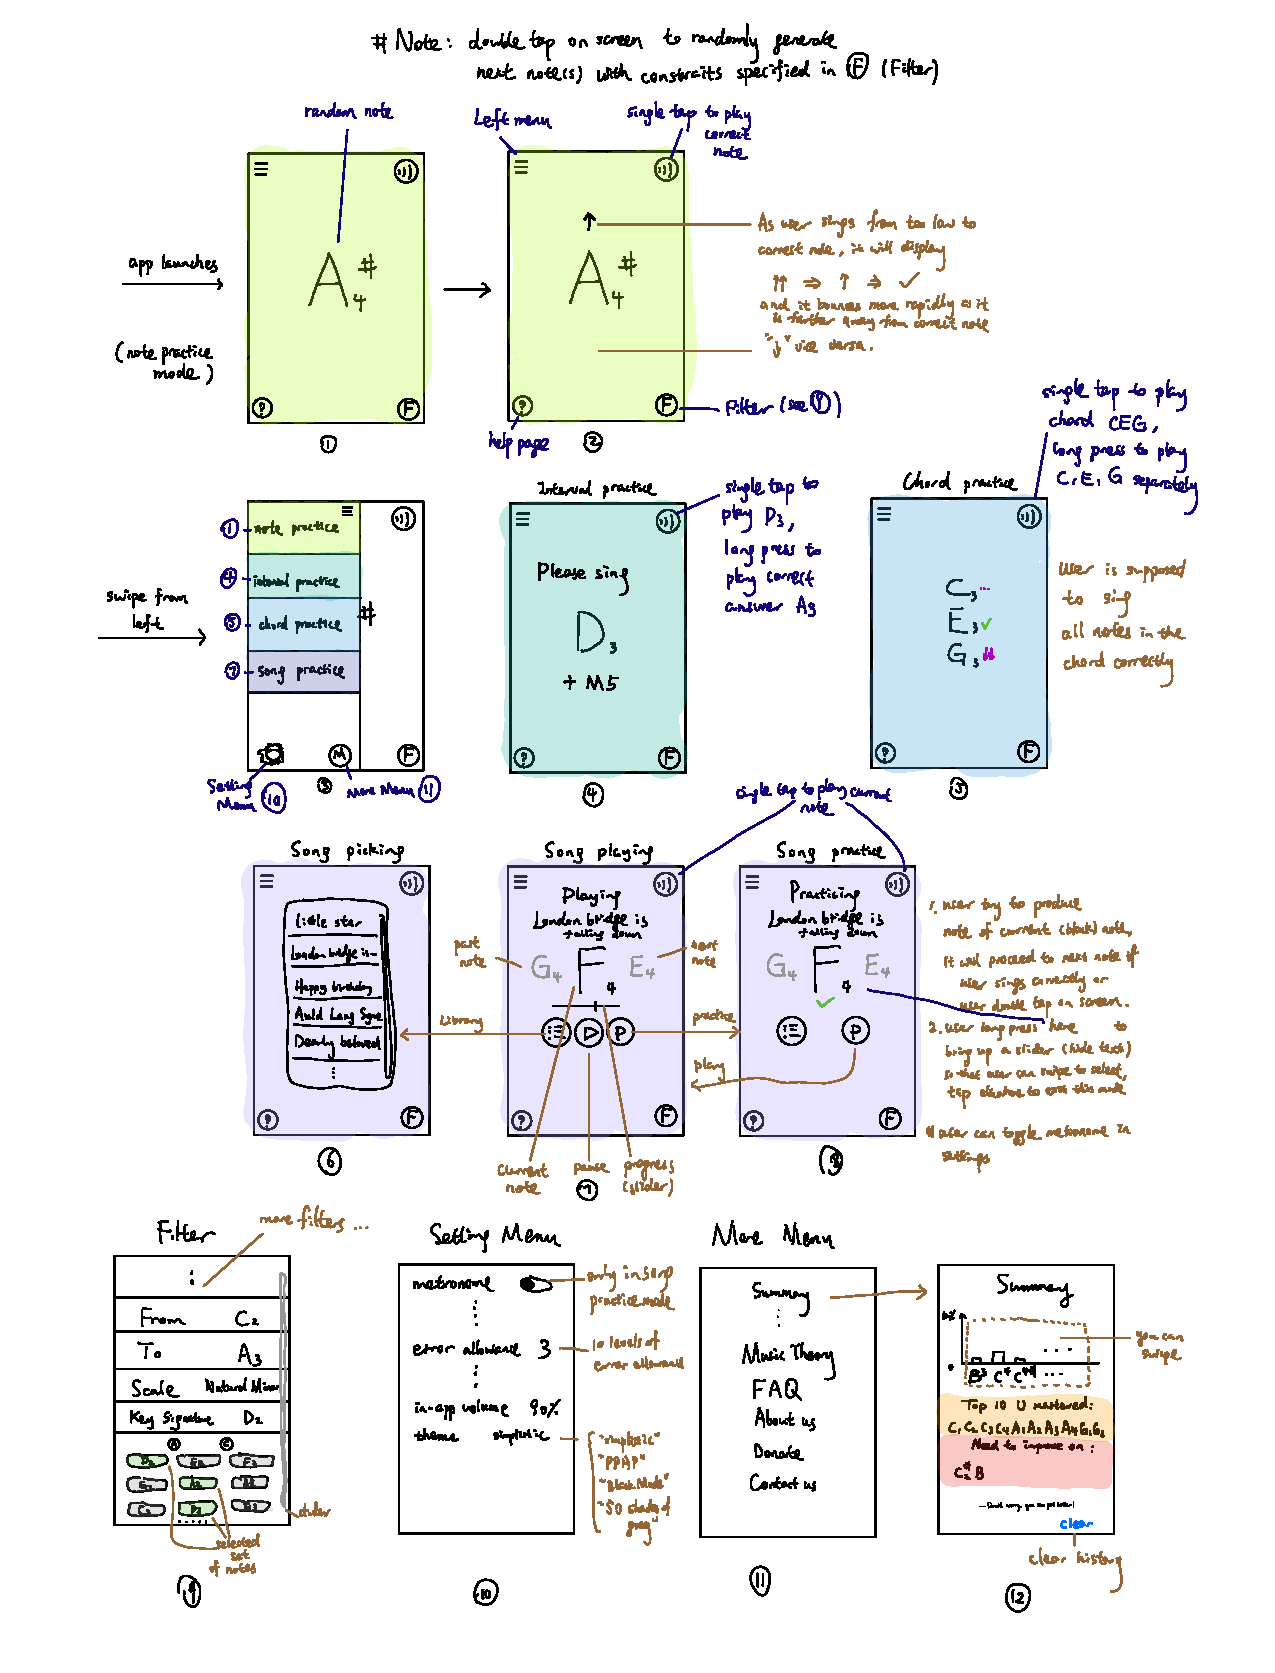
\includepdf[pages={1}]{./wireframes.pdf}

\end{document}
